In questo capitolo analizzeremo diversi concetti matematici essenziali nella risoluzione numerica di simulazioni CFD e,
in particolare, della simulazione oggetto di questa tesi. In particolare ci soffermeremo sulle equazioni utilizzate
per simulare correttamente il movimento del gas e delle particelle all'interno dell'ugello.

\section{Equazioni differenziali alle derivate parziali}\label{PDE}
In analisi matematica per \textit{Equazione differenziale alle derivate parziali} (PDE in breve) intendiamo una qualsiasi equazione differenziale
che coinvolge derivate parziali di una funzione incognita con più variabili indipendenti.
Invece di scrivere esplicitamente la funzione essa viene definita indirettamente attraverso una relazione fra se stessa
e le sue derivate parziali. La relazione deve necessariamente essere locale, ovvero deve connettere la funzione alle sue derivate nello stesso punto.

Solitamente le PDE vengono utilizzate per risolvere complessi problemi in svariati campi fisici tra cui:
\begin{itemize}
    \item Elettrostatica
    \item Elettrodinamica
    \item Meccanica dei fluidi
    \item Aereodinamica
    \item Elasticità
    \item Meccanica Quantistica
    \item Relatività
\end{itemize}

Un equazione differenziale alle derivate parziali di ordine \(k\) ha la seguente forma:
\begin{equation}
    F(D^ku(x),D^{k-1}u(x),...,Du(x),u(x),x)=0
\end{equation}
dove \(k\) rappresenta un numero intero, \(D^k\) un operatore di derivazione di ordine \(k\) rispetto a una o più variabili e infine
\(x\) appartiene a un sottoinsieme \(U\) aperto di $\mathbb{R}^n$.
La funzione \(F\) è data, mentre la funzione \(u\) è l'incognita dell'equazione.
La risoluzione di una PDE consiste nella ricerca di tutte le funzioni \(u\) che la rendono un'identità su un opportuno insieme.
Di solito viene anche richiesto che la soluzione soddisfi una o più condizioni al contorno ausiliarie.
Le PDE possono essere anche non lineari, quando dipende non-linearmente dal più alto grado di derivazione presente.
\section{Equazioni di Navier-Stokes}\label{navierstokes}
In ambito di fluidodinamica le equazioni (PDE) di Navier-Stokes sono un sistema di tre equazioni, dette di bilancio, della meccanica dei corpi continui.
Esse descrivono un flusso lineare viscoso e fanno parte dei cosiddetti 7 problemi per il millennio, ovvero problemi la cui difficoltà intrinseca li rende estremamente complessi da risolvere.
Difficilmente si possono raggiungere soluzioni analitiche esatte (solo in casi di problemi semplificati), solitamente ci si affida a soluzioni approssimate per i problemi comuni.

    \subsection{Modello matematico}
    Le equazioni di Navier-Stokes introducono termini come viscosità e conducibilità termica del fluido all'interno delle altrettanto celebri equazioni di bilancio di Eulero,
    che complicano la soluzione e diminuiscono l'efficienza predittiva delle stesse. Nel caso generale infatti il sistema coinvolge cinque PDE con venti variabili.

    Possiamo utilizzare le equazioni di Navier-Stokes per descrivere completamente qualsiasi flusso fluido, anche in presenza di turbolenze.
    Nel caso di flusso turbolento le traiettorie di particelle di flusso non sono più costanti nel tempo.
    Le risorse di calcolo necessarie alla risoluzione di queste traiettorie crescono in base al numero di Reynolds (numero adimensionale usato in fluidodinamica, proporzionale al rapporto tra le forze d'inerzia
    e le forze viscose di un fluido) in maniera esponenziale. Le equazioni vengono completate dalle condizioni al contorno e dalle condizioni iniziali.
    La soluzione a queste equazioni fornisce informazioni sul campo delle velocità del fluido, dalle quali poi si può risalire alle restanti grandezze.

    Le equazioni che descrivono il moto di un fluido a densità costante $\rho$, in un dominio $\Omega  \subset  \mathbb{R}^d$ (with $d = 2, 3$),
    sono scritte nella seguente forma:
    \begin{alignat}{2}
        &\frac{\partial \boldsymbol{u}}{\partial t} +
        \left(\boldsymbol{u} \cdot \nabla \right) \boldsymbol{u} -
        \nabla \cdot \tau + \nabla p
        =
        \boldsymbol{f}, \,\,\,\,\,\, &&\forall \boldsymbol{x} \in \Omega, t > 0, \label{eq:ns_mom}\\
        %
        &\nabla \cdot \boldsymbol{u} = 0, \,\,\,\,\,\, &&\forall \boldsymbol{x} \in \Omega, t > 0, \label{eq:ns_cont}
    \end{alignat}
    dove $\boldsymbol{u}$ è la velocità del flusso, $\rho$ è la densità del flusso, $p$ è la pressione del flusso divisa per la densità,
    $\nu = \mu / \rho$ la viscosità cinematica, $\mu$ la viscosità dinamica, $\boldsymbol{f}$ la forza per unità di massa e $\tau$ rappresenta lo stress viscoso ed è equivalente a:
    $\tau = 2\mu\varepsilon$ con $\varepsilon=\frac{1}{2}\left(\nabla\boldsymbol{u}\cdot\nabla\boldsymbol{u}^\top\right)$.
    La prima equazione del sistema è l'equazione di bilancio del momento \eqref{eq:ns_mom},
    la seconda è l'equazione di conservazione della massa \eqref{eq:ns_cont},
    chiamata anche come equazione di continuità. Il temine $\left(\boldsymbol{u} \cdot \nabla \right) \boldsymbol{u}$ descrive il processo di trasporto convettivo,
    mentre $-\nabla \cdot \tau$ descrive il processo di diffusione molecolare.
    Nel caso in cui la densità sia costante, usando l'equazione di continuità, otteniamo
    \begin{equation}
    \nabla \cdot \tau = 2\mu\nabla \cdot \varepsilon = \mu\nabla \cdot \left(\nabla\boldsymbol{u} + \nabla\boldsymbol{u}^\top \right) = \mu\nabla^2\boldsymbol{u}
    \end{equation}
    e il sistema può essere scritto nella forma compatta:
    \begin{alignat}{2}
        &\frac{\partial \boldsymbol{u}}{\partial t} +
        \left(\boldsymbol{u} \cdot \nabla \right) \boldsymbol{u} -
        \nu \Delta \boldsymbol{u} + \nabla p
        =
        \boldsymbol{f}, \,\,\,\,\,\, \qquad &&\forall \boldsymbol{x} \in \Omega, t > 0, \label{eq:ns_mom_2}\\
        %
        &\nabla \cdot \boldsymbol{u} = 0, \,\,\,\,\,\, &&\forall \boldsymbol{x} \in \Omega, t > 0. \label{eq:ns_cont_2}
    \end{alignat}
    Le equazioni \eqref{eq:ns_mom_2} e \eqref{eq:ns_cont_2} sono chiamate equazioni incomprimibili di Navier-Stokes.
    Generalmente, i flussi che soddisfano queste condizioni di incompressibilità $\nabla \cdot \boldsymbol{u} = 0$, sono chiamati fluidi incompressibili.
    Come anticipato è necessario aggiungere delle condizioni iniziali per impostare correttamente il problema, tali sono:
    \begin{equation}
        \label{eq:ns_init}
        \boldsymbol{u}\left(\boldsymbol{x},0 \right) = \boldsymbol{u}_0\left(\boldsymbol{x} \right) \,\,\,\, \forall \boldsymbol{x} \in \Omega
    \end{equation}
    con le relative condizioni al contorno:
    \begin{alignat}{2}
        &\boldsymbol{u}\left(\boldsymbol{x},t \right) = \boldsymbol{u}_D\left(\boldsymbol{x},t \right) \label{eq:ns_bound_1}\,\,\,\, &&\forall \boldsymbol{x} \in \Gamma_D, \\
        &\left(\nu \frac{\partial \boldsymbol{u}}{\partial \boldsymbol{n}} - p \boldsymbol{n} \right)\left(\boldsymbol{x},t \right) = \boldsymbol{t}\left(\boldsymbol{x},t \right) \label{eq:ns_bound_2}\,\,\,\, \qquad &&\forall \boldsymbol{x} \in \Gamma_N,
    \end{alignat}
    Le equazioni \eqref{eq:ns_mom_2} e \eqref{eq:ns_cont_2} sono generalmente più semplici da risolvere da un punto di vista computazionale, sono quindi quelle su cui si basa
    il modello matematico del simulatore oggetto della tesi.

\section{Metodo elementi finiti}\label{fem}
Il metodo degli elementi finiti, o \textbf{FEM} dall'inglese \textit{finite element method}, è una tecnica numerica
che cerca soluzioni approssimate a problemi descritti da PDE (\label{PDE}).
Compete con altri metodi ben noti quali: metodo delle differenze finite, metodo dei volumi finiti, metodo degli elementi al contorno,
metodo delle celle, metodo spettrale ma rimane tuttora il più utilizzato in ambito computazionale.
Questo metodo si presta soprattutto a problemi dettati da PDE aventi domini di forma complessa o variabile, quando il livello di accuratezza
richiesto non è omogeneo sul dominio (si veda in \ref{mesh} l'accuratezza in prossimità dell'ugello) e quando la soluzione cercata pecca di regolarità.
Il metodo FEM è anche utilizzato per discretizzare il problema dei flussi incomprimibili visto nella precedente sezione, ed è alla base della soluzione implementata in questa tesi.

In generale questi metodi prevedono la discretizzazione di un dominio in griglie o mesh di punti in cui computare soluzioni basate su discreti step temporali.
Su ciascun elemento del dominio discretizzato viene espressa una combinazione lineare di funzioni dette funzioni forma, o shape functions, che spesso vengono approssimate.
L'accuratezza delle soluzioni trovate per queste funzioni è legata al grado del polinomio che le compone.

Il metodo degli elementi finiti fa parte della classe del metodo di Galërkin, metodi di analisi numerica che permettono di passare da uno spazio continuo a uno discreto, il cui punto di partenza
è la cosiddetta formulazione debole di un problema differenziale. La formulazione debole è essenziale poiché richiede alla soluzione di soddisfare determinati requisiti di regolarità,
che sono realistiche per quasi tutti i problemi d'ingegneria a cui si applicano. I metodi di tipo Galërkin approssimano la soluzione del problema scritto in forma debole mediante
la combinazione lineare delle funzioni di forma elementari. I coefficienti di queste combinazioni lineari sono i gradi di libertà del problema che rappresentano le incognite del problema ottenuto dalla discretizzazione.

    \subsection{Esempio FEM con un grado di libertà}
    Proponiamo di seguito un esempio di problema risolvibile con FEM \cite{HughesThomasJ.R2000Tfem}:
    $u_{,xx} + f = 0$
    la virgola indica la differenziazione mentre f è una funzione continua
    e derivabile nell'intervallo $\left[0,1\right]$. Un problema ai limiti richiede
    l'imposizione di alcune condizioni al contorno sulla funzione $u$, supponiamo quindi:
    \begin{equation}
        u(1) = q \text{e} -u_{,x}(0)=h
    \end{equation}
    Con $q$ e $e$ costanti. La formula forte del problema sarà dunque la seguente:
    \begin{equation}
        \text { (S) }\left\{\begin{array}{l}
        \text { Dati } f: \bar{\Omega} \rightarrow \mathbb{R} \text { e le costanti } q \text { e } h, \text { trovare } u: \bar{\Omega} \rightarrow \mathbb{R}, \text { tale che } \\
        \qquad
        \begin{array}{c}
        u_{, x x}+f=0 \\
        u(1)=q \\
        -u_{, x}(0)=h \\
        \end{array} \\
        \end{array}\right.
    \end{equation}
    Dove $\Omega$ appartiene all'intervallo aperto tra 0 e 1, mentre $\bar{\Omega}$ al
    medesimo chiuso.
    La soluzione esatta è:
    \begin{equation}
        u(x)=q+(1-x) h+\int_{x}^{1}\left\{\int_{0}^{y} f(z) d z\right\} d y
    \end{equation}
    dove con $y$ e $z$ indichiamo delle variabili di comodo.
    Per definire la forma debole di $S$ definiamo due classi di funzioni:
    \begin{itemize}
        \item \textit{Soluzioni di prova}, indicate con $S$, tali per cui:
        \begin{equation}
            \mathcal{S}=u \mid u \in H^{1}, u(1)=q
        \end{equation}
        \item \textit{Funzioni peso}, indicate con $\mathcal{V}$, tali per cui:
        \begin{equation}
            \mathcal{V}=w \mid w \in H^{1}, w(1)=0
        \end{equation}
    \end{itemize}
    Ciò detto, è possibile definire la formulazione debole:
    \begin{equation}
        (W)\left\{\begin{array}{l}
        \text { Dati } f, q, \text { e } h \text { come prima, trovare } u \in \mathcal{S}, \text { tale che per ogni } w \in \mathcal{V} \\
        \qquad \int_{0}^{1} w_{, x} u_{, x} d x=\int_{0}^{1} w f d x+w(0) h
        \end{array}\right.
    \end{equation}

    Le formulazioni, debole e forte, sono equivalenti, perciò per ottenere una soluzione
    valida, pur sempre approssimata, il metodo degli elementi finiti considera la formulazione
    debole. Come citato in precedenza un modo per ottenere tale soluzione è attraverso
    il \textit{metodo di Galerkin}.
    In primis procediamo alla costruzione delle approssimazioni di dimensione finita
    $\mathcal{S}^{h} \subset \mathcal{S}$ e $\mathcal{V}^{h} \subset \mathcal{V}$.
    Quindi per ogni $v^{h} \in \mathcal{V}^{h}$ costruiamo una funzione
    $u^h \in \mathcal{S}^h$:
    \begin{equation}
        a(w^h,u^h) = (w^h,f) + w^h(0)h
    \end{equation}
    Quest'ultima definisce una soluzione approssimata $u^h$.
    Sostituendo la precednete, definiramo la forma di Galerkin del problema:
    \begin{equation}
        \text { (G) }\left\{\begin{array}{l}
        \text { Dati } f, q, \text { e } h \text { come prima, trovare } u^{h}=v^{h}+q^{h}, \text { dove } v^{h} \in \mathcal{V}^{h} \\
        \text { tale che per ogni } w^{h} \in \mathcal{V}^{h} \\
        \qquad a\left(w^{h}, v^{h}\right)=\left(w^{h}, f\right)+w^{h}(0) h-a\left(w^{h}, q^{h}\right)
        \end{array}\right.
    \end{equation}
    Riscrivibile come:
    \begin{equation}
        \sum_{B=1}^{n} a\left(N_{A}, N_{B}\right) d_{B}=\left(N_{A}, f\right)+N_{A}(0) h-a\left(N_{A}, N_{n+1} q\right)
    \end{equation}
    Dove $N_A$,$N_B$ e $N_{n+1}$ sono dette funzioni di forma, per le quali
    $N_A(1)=0$, $N_B(1)=0$, $N_{n+1}(1)=1$. Ciò rappresenta un sistema di
    $n$ equazioni in $n$ incognite, che possiamo riscrivere come:
    \begin{equation}
        \sum_{B=1}^{n} K_{A B} d_{B}=F_{A}, \quad A=1,2, \ldots, n
    \end{equation}
    Dove:
    \begin{equation}
        \begin{array}{c}
        K_{A B}=a\left(N_{a}, N_{b}\right) \\
        F_{A}=\left(N_{A}, f\right)+N_{A}(0) h-a\left(N_{A}, N_{n+1} q\right)
        \end{array}
    \end{equation}
    Definiamo ora le matrici:
    \begin{equation}
        \begin{aligned}
        K=\left[K_{A B}\right] &=\left[\begin{array}{ccc}
        K_{11} & \ldots & K_{1 n} \\
        \vdots & & \vdots \\
        K_{n 1} & \ldots & K_{n n}
        \end{array}\right]
        \end{aligned}
    \end{equation}
    \begin{equation}
        \begin{aligned}
        F &=\left\{F_{A}\right\}=\left\{\begin{array}{c}
        F_{1} \\
        \vdots \\
        F_{n}
        \end{array}\right\}
    \end{aligned}
\end{equation}
\begin{equation}
    \begin{aligned}
        d=\left\{d_{B}\right\}=\left\{\begin{array}{c}
        d_{1} \\
        \vdots \\
        d_{n}
        \end{array}\right\}
    \end{aligned}
\end{equation}
    Riformulando il problema di Galerkin in:
    \begin{equation}
        \text { (M) }\left\{\begin{array}{l}
        \text { Date la matrice di coefficienti } K \text { e il vet tore } F, \text { trovare } d \text { tale che } \\
        \qquad K d=F
        \end{array}\right.
        \end{equation}

        Per un'applicazione 1D: si prenda $n=1$, allora
        $w^h=c_1N_1,eu^h=v^h+q^h = d_1N_1+qN_2$. L'unica incognita è $d1$. Le funzioni
        di forma devono soddisfare $N_1(1)=0$ e $N_2(1)=0$. Prendiamo $N_1(x)=1-x$ e $N_2(x)$.
        Le matrici introdotte in precedenza diventano quindi:
        \begin{equation}
            \begin{array}{c}
            K=\left\{K_{11}\right\}=K_{11}=a\left(N_{1}, N_{1}\right)=\int_{0}^{1} N_{1, x} N_{1, x} d x=1 \\
            F=\left\{F_{1}\right\}=F_{1}=\left(F_{1}, f\right)+N_{1}(0) h-a\left(N_{1}, N_{2}\right) q \\
            =\int_{0}^{1}(1-x) f(x) d x+h-\int_{0}^{1} N_{1, x} N_{2, x} d x q=\int_{0}^{1}(1-x) f(x) d x+h+q \\
            d=\left\{d_{1}\right\}=d_{1}=K_{11}^{-1} F_{1}=F_{1}
            \end{array}
        \end{equation}
        Di conseguenza:
        \begin{equation}
            u^{h}(x)=d_{1}(1-x)+q x
        \end{equation}
        Se $f=0$:
        \begin{equation}
            u^{h}(x)=u(x)=q+(1-x) h
        \end{equation}
        In questo caso la soluzione approssimata è esatta.
        Se $f$ è uguale a una costante $f(x)=p$:
        \begin{equation}
            \begin{array}{l}
            u_{\text {part}}(x)=\frac{p\left(1-x^{2}\right)}{2} \\
            u_{\text {part}}^{h}(x)=\frac{p(1-x)}{2}
            \end{array}
        \end{equation}
        Se invece $f(x)=qx$, dove $q$ è una costante, allora avremo:
        \begin{equation}
            \begin{aligned}
            u_{\text {part}}(x) &=\frac{q\left(1-x^{3}\right)}{6} \\
            u_{\text {part}}^{h}(x) &=\frac{q(1-x)}{6}
            \end{aligned}
        \end{equation}
        \begin{figure}[H]
            \centering
            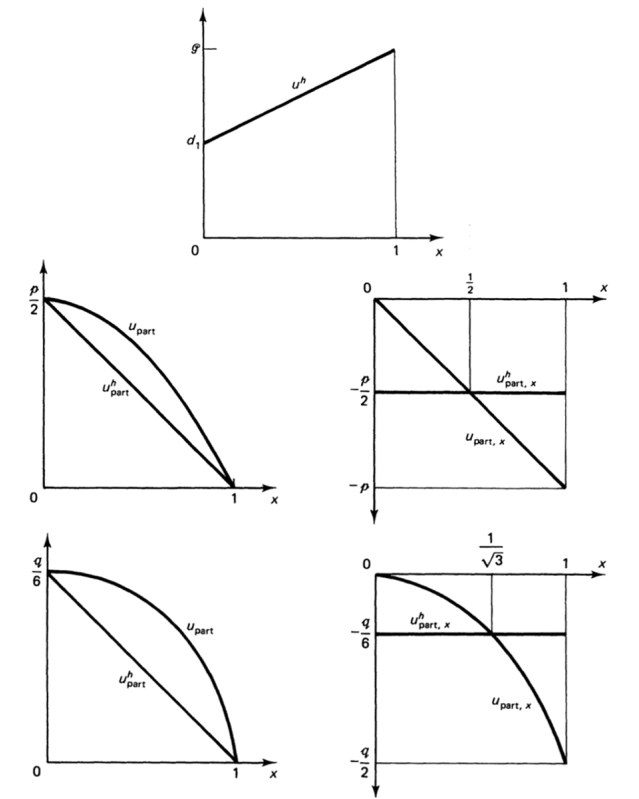
\includegraphics[width=\linewidth]{figure/galerkin.png}
            \caption{Soluzioni dell'esempio, in alto la soluzione di Galerkin nel primo caso, al
            centro e in basso un confronto tra la soluzione esatta e quella di Galerkin nel secondo e
            nel terzo caso. \cite{HughesThomasJ.R2000Tfem}}
        \end{figure}
\section{Metodo Newton-Raphson}\label{newtonraphson}
Il metodo Newton-Raphson, detto anche metodo delle tangenti, è uno dei metodi utilizzati per calcolare approssimativamente la soluzione di un equazione nella forma:
\begin{equation}
    f(x) = 0
\end{equation}
Il metodo consiste nel sostituire a una generica curva \(y = f(x)\) la tangente alla curva stessa, partendo da un qualsiasi punto.
La relazione di ricorrenza del metodo è la seguente:
\begin{equation}
    x_{n+1} = x_n - \frac{f(x_n)}{df(x_n)}
\end{equation}
dove \(n\) rappresenta il numero di approssimazioni.
Questo metodo è stato utilizzando principalmente per approssimare le soluzioni delle funzioni di forma, nel modulo di Navier-Stokes (\ref{5:navierstokes}).